\documentclass{article}
\usepackage{multicol}
\usepackage[margin=0.5in]{geometry}
\usepackage{amssymb}
\usepackage{enumerate}
\usepackage{amsmath}
\usepackage{mathtools}
\usepackage{graphicx}

%\usepackage{macros}
\usepackage{fancyvrb}
\DefineVerbatimEnvironment{code}{Verbatim}{fontsize=\small}
\DefineVerbatimEnvironment{example}{Verbatim}{fontsize=\small}

\begin{document}
\small
\begin{multicols}{2}
  \raggedright
  {\bf Files and Directories}

  {\tt int open(char* pathname, int flags)}. Some useful flags:
  {\tt O\_WRONLY, O\_RDONLY, O\_CREAT, O\_EXCL}. Returns file descriptor. -1 on
  error. Can also pass a third parameter of the desired mode for the file (see
  below for mode flags).

  {\tt ssize\_t read(int fd, void* buf, size\_t count)} Read up to {\tt count}
  bytes from the fd into buf. Returns the number of bytes read or -1 if error.

  {\tt ssize\_t write(int fd, const void* buf, size\_t count)} write up to {\tt
  count} bytes into the fd from buf. Returns the number of bytes written or -1
  if error.

  {\tt int close(fd)} returns 0 on success.
  In general, \texttt{FILE *} (opened with \texttt{fopen}) and C++
  \texttt{iostream}s have a more powerful API, but only generalize to stdio and
  local files. File descriptors have a less powerful API but also generalize to
  network streams.

  {\tt DIR* opendir(char* path)},
  {\tt struct dirent* readdir(DIR* dir)}: \texttt{struct dirent*} represents an
  entry (file or subdirectory) inside a directory, where \texttt{d\_ino} and
  \texttt{d\_name} fields are definitely present on all platforms.
  {\footnotesize
  \begin{verbatim}
struct dirent {
  ino_t          d_ino;       /* inode number */
  off_t          d_off;       /* offset to the next dirent */
  unsigned short d_reclen;    /* length of this record */
  unsigned char  d_type;      /* type of file; not supported
                                 by all file system types */
  char           d_name[256]; /* filename */
};\end{verbatim}}
  \texttt{readdir} should be called several times to list all \texttt{dirent}s,
  then it will return \texttt{NULL} to signal all have been read. Then
  \texttt{int closedir(DIR* dirp)} should be called to free the dir pointer.

  {\tt stat} populates a {\tt struct stat}: use macros
  {\tt S\_ISREG, S\_ISDIR, S\_ISLINK(st.st\_mode) } on the mode field to see
  what type of object it is. Bitwise-and the mode with \texttt{S\_IRUSR},
  \texttt{S\_IWUSR}, \texttt{S\_IXUSR}, \texttt{S\_IRGRP}, \texttt{S\_IROTH},
  etc. to check permissions.
  {\tt stat(char* path, struct stat *st)} populates \texttt{struct stat} defined
  as
  {\footnotesize
  \begin{verbatim}
struct stat {
  dev_t     st_dev;     /* ID of device containing file */
  ino_t     st_ino;     /* inode number */
  mode_t    st_mode;    /* protection */
  nlink_t   st_nlink;   /* number of hard links */
  uid_t     st_uid;     /* user ID of owner */
  gid_t     st_gid;     /* group ID of owner */
  dev_t     st_rdev;    /* device ID (if special file) */
  off_t     st_size;    /* total size, in bytes */
  blksize_t st_blksize; /* blocksize for file system I/O */
  blkcnt_t  st_blocks;  /* number of 512B blocks allocated */
  time_t    st_atime;   /* time of last access */
  time_t    st_mtime;   /* time of last modification */
  time_t    st_ctime;   /* time of last status change */
}; \end{verbatim}}
  {\tt lstat} Same as {\tt stat} except {\tt lstat} returns info about the
  link while {\tt stat} returns info about the linked file if a file is a link.

  {\tt int dup2(int oldfd, int newfd)} makes new fd point to oldfd, closing new
  if necessary. For example, {\tt dup2(fd, STDIN\_FILENO)} to dump fd into STDIN.

  \texttt{int pipe(int pipefd[2])} makes a data channel (pipe) between two fds:
  \texttt{pipefd[0]} is the read end, \texttt{pipefd[1]} is the write end.
  Anything written to the write end will be buffered until read by the read end.
  {\scriptsize
  \begin{verbatim}
typedef struct subprocess_t {
  pid_t pid;
  int infd;
  int outfd;
} subprocess_t;
subprocess_t subprocess_open(const char *command) {
  int pcfds[2]; // parent-to-child descriptors
  int cpfds[2]; // child-to-parent descriptors
  pipe(pcfds); pipe(cpfds);
  subprocess_t process = { fork(), pcfds[1], cpfds[0] };
  if (process.pid == 0) {
    dup2(pcfds[0], STDIN_FILENO); dup2(cpfds[1], STDOUT_FILENO);
    close(pcfds[0]); close(cpfds[0]); close(pcfds[1]); close(cpfds[1]);
    char *argv[] = {"/bin/sh", "-c", (char *) command, NULL};
    execvp(argv[0], argv);
  }
  close(pcfds[0]); close(cpfds[1]);
  return process;
}
int subprocess_close(subprocess_t sp) {
  int status;
  pid_t pid = waitpid(sp.pid, &status, WNOHANG | WUNTRACED);
  return pid == sp.pid && WIFEXITED(status) ? WEXITSTATUS(status) : -1;
}
\end{verbatim}}

  \noindent\rule{4cm}{0.4pt}

  {\bf Layering and Naming}
  Block $\rightarrow$ File $\rightarrow$ Inode number $\rightarrow$ File name
  $\rightarrow$ Path name $\rightarrow$ Absolute path name $\rightarrow$
  Symbolic link

  Block to Inode are machine-oriented. File name is machine-user interface. Rest
  are user-oriented.

  Three parts to a naming scheme: namespace (all possible names), name-mapping
  algorithm (some names to values in ``universe of values''), ``universe of
  values'' (a value you map to). Like Domain-name system: namespace=domain names
  (www.google.com), mapping=domain name resolution, universe=ip addresses.

  Modularity between layers. %TODO

  \noindent\rule{4cm}{0.4pt}

  {\bf v6 Data structures}
  \begin{verbatim}
struct inode {
  uint16_t i_mode; //bit vec of file type and permissions
  uint8_t i_nlink	//number of directory entries
  uint8_t i_uid; //owner
  uint8_t i_gid; //group of owner
  uint8_t i_size0; //most significant byte of size
  uint16_t i_size1; //lower two bytes if size (of 3 bytes)
  uint16_t i_addr[8]; //device addresses constituting file
  uint16_t i_atime[2]; //access time
  uint16_t i_mtime[2]; // modify time
};

struct filsys {
  uint16_t s_isize; // size in blocks of I list
  uint16_t s_fsize; // size in blocks of entire volume
  uint16_t s_nfree; // number of in core free blocks (0-100)
  uint16_t s_free[100]; // in core free blocks
  uint16_t s_ninode; // number of in core I nodes (0-100)
  uint16_t s_inode[100]; // in core free I nodes
  uint8_t s_flock; // lock during free list manipulation
  uint8_t s_ilock; // lock during I list manipulation
  uint8_t s_fmod; // super block modified flag
  uint8_t s_ronly; // mounted read-only flag
  uint16_t s_time[2]; // current date of last update
  uint16_t pad[48]; // aligns struct filesys to be
  // 512 bytes in size (the block size!)
};

struct direntv6 {
  uint16_t d_inumber;
  char     d_name[14];
};
  \end{verbatim}

  \noindent\rule{4cm}{0.4pt}

  {\bf Processes}

  {\tt pit\_t fork()} called once, returns twice. {\tt pid = 0} if in child
  process.

  {\tt waitpid(pid\_t pid, int *status, int options)} store status info into\\
  {\it status}: {\tt WIFEXITED(status), WEXITSTATUS, WIFSIGNALED, WTERMSIG,
  WCOREDUMP, WIFSTOPPED} need untraced, {\tt WSTOPSIG} number of signal that
  stopped the child (if ifstopped returned true), {\tt WIFCONTINUED} child
  resumed by
  sigcont.\\
  {\it Pid}: $<-1$ (wait for any child process whose process group ID is equal to the
  absolute value of pid.), $-1$ (wait for any child process), $0$ (wait for any
  child process whose process group ID is equal to that of the calling process),
  $>0$ (wait for that specific pid)\\
  {\it Options}: {\tt WNOHANG} (return immediately if no child has exited), {\tt
  WUNTRACED} (return if a child has stopped even if not traced by ptrace) {\tt
  WCONTINUED} (return if a stopped child has been resumed by delivery of
  \texttt{SIGCONT}).

  {\tt int execvp(const char* path, char* argv[])} Consumes the process on
  success so it should not be expected to return.
\begin{verbatim}
pid_t pid = fork();
exitIf(pid == -1, kForkFailed, stderr,
  "fork function failed.\n");
if (pid == 0) {
  if (execvp(argv[0], argv) < 0) {
    printf("%s: Command not found\n", argv[0]);
    exit(0);
  }
}\end{verbatim}

  {\tt int signal(int signum, (void sighandler(int signum)))}. If process gets
  {\tt signum}, it calls the sighandler. \texttt{SIGCHLD} is received if a child
  process that has been previously forked off finishes running. \texttt{SIGINT}
  is interruption (ctrl-C). \texttt{SIGKILL} is when the process is killed by
  \texttt{kill} to make it stop immediately (can't be caught), \texttt{SIGTERM}
  is the same but lets it clean up. \texttt{SIGSTOP} is temporary stopping
  (ctrl-Z), \texttt{SIGCONT} is continuation after stopping, perhaps by
  \texttt{fg} or \texttt{bg}.

  {\it Signal handlers} are functions that return voids. Need to use global (no
  state).
  \begin{verbatim}
static void reapChild(int sig) {
pid_t pid;
while (true) {
  pid = waitpid(-1, NULL, WNOHANG);
  if (pid <= 0) break;
  numChildrenDonePlaying++;
} \end{verbatim}
  {\it Signal blocking} Useful for handling \texttt{SIGCHLD}s etc only after they, as
  jobs, have been added to a list or something, so proper concurrency can
  happen.
  \begin{verbatim}
  sigset_t mask;
  sigemptyset(&mask);
  sigaddset(&mask, SIGCHLD);
  sigprocmask(SIG_BLOCK, &mask, NULL);
  // critical region
  sigprocmask(SIG_UNBLOCK,&mask,NULL);\end{verbatim}

  {\tt int kill(pid\_t pid, int sig)} Sends sig to process pid. 0 success, -1
  error.

  {\it Process ids} %TODO?

  {\it Process groups} A parent will create a group with its child -- so can
  send signals to all of its children.

  {\it Interprocess Concurrency} Use blocking to handle signals only when
  possible. Use pipes to handle communications.

  \noindent\rule{4cm}{0.4pt}

  {\bf Threading}
  Threads have independent stacks, but they all share access to the same text,
  data, and heap segments. Stack segment is subdivided into multiple miniature
  stacks. Thread manager time slices and switches between simultaneously running
  threads in much the same way that the kernel scheduler switches between
  processes.
  {\it Pro}\\
  - Easier to support communication between threads, because address spaces
  accessible are largely the same.\\
  - Multiple threads can access the same global data and one copy of the code.\\
  - One thread can share its stack space (via pointers and references) with
  another thread.\\
  {\it Con}\\
  - Multiple threads must unfortunately access the same global data and only one
  copy of the code.\\
  - Every thread might share its stack space (via pointers and references) with
  another thread.

  {\tt pthread\_t pthread\_create(pthread\_t *pt, const pthread\_attr\_t *attr,
  void* (routine)(void* args))}. Can pass arguments in the void *args.\\
  {\tt pthread\_join(pthread\_t thread, void **retval)} waits for thread to
  terminate. Returns 0 on success, else returns error number. Copies return
  value into void **retval.

  {\it Race conditions}

  {\it Critical regions}

  {\tt thread t = thread((void *) (thread function)(arg1, arg2, \ldots))} Use
  {\tt t.detach()} to detach thread and have it run on its own. Use {\tt
  t.join()} to join.

  \noindent\rule{4cm}{0.4pt}

  {\bf Locking}

  {\tt mutex m}, {\tt m.lock()}, {\tt m.unlock()}

  {\tt lock\_guard<mutex> lg(m)}. Constructor locks it. Destructor unlocks it.

  {\tt unique\_lock<mutex> ul(m, defer\_lock)}. Wraps around anything with
  lock/unlock. Used for condition variables.

  {\tt condition\_variable cv}, {\tt cv.wait(ul, bool (function()))}. Checks if
  function returns true. If false, unlocks ul, waits to be notified to check
  function again. {\tt cv.notify\_all()} notifies every instance of cv that is
  waiting.

  {\tt semaphore s(int value).} Atomic counter of a shared resource. No
  get-value since value could change. No copy constructor. {\tt
  s.signal()} signals resource added (increment/\texttt{++}), {\tt s.wait()}
  blocks until there is at least one variable. No busy waiting!

  {\it Rendezvousing etc\ldots} Reader/Writer example.
  \begin{verbatim}
static const unsigned int kNumBuffers = 30;
static const unsigned int kNumCycles = 4;
static char buffer[kNumBuffers];
static semaphore emptyBuffers(kNumBuffers);
static semaphore fullBuffers(0);
static void writer() {
  for (unsigned int i = 0;
  i < kNumCycles * kNumBuffers; i++) {
    char ch = prepareData();
    // don't try to write to a
    // slot unless you know it's empty
    emptyBuffers.wait();
    buffer[i % kNumBuffers] = ch;
    // signal reader more to read
    fullBuffers.signal();
  }
}
static void reader() {
  for (unsigned int i = 0;
  i < kNumCycles * kNumBuffers; i++) {
    // don't try to read from a
    // slot unless you know it's full
    fullBuffers.wait();
    char ch = buffer[i % kNumBuffers];
    // signal writer there is open slot for data
    emptyBuffers.signal();
    processData(ch);
  }
}
int main(int argc, const char *argv[]) {
  thread w(writer);
  thread r(reader);
  w.join();
  r.join();
  return 0;
} \end{verbatim}
\noindent\rule{4cm}{0.4pt}

  {\bf Networking}

  {\it Client-server model} Servers wait by a phone (socket), bound to a port,
  and listens for incomming requests to accept as they come in.

  {\it {\tt gethostbyname} vs. {\tt gethostbyname\_r}}
  {\tt struct hostent *gethostbyname(const char *name)} feed in
  ``www.google.com'' to get a hostent.

  The \_r version is the reentrant version. It is thread safe with a complicated
  signature!

  {\tt int getaddrinfo(const char *hostname, const char *servname,
  const struct addrinfo *hints, struct addrinfo **res);
  void freeaddrinfo(struct addrinfo *ai);} implants the head of a
  linked list of struct addrinfo records in the space addressed by
  res.\\
  {\tt freeaddrinfo(struct addrinfo *ai)} fully disposes of the linked list
  surfaced by an earlier call to getaddrinfo.\\
  {\tt int getnameinfo(const struct sockaddr *sa, socklen\_t salen,
  char *host, socklen\_t hostlen,
  char *serv, socklen\_t servlen, int flags);} gets ip address info.

  {\tt struct hostent *gethostbyaddr(const char *addr, int len, int type);}

  {\tt sock\_addr}

  \noindent\rule{4cm}{0.4pt}

  {\bf Socket API calls}

  {\tt int socket(int socket\_family, int socket\_type, int protocol)}

  {\tt int bind(int sockfd, const struct sockaddr *addr, socklen\_t addrlen)}
  assigns the address specified by addr to the socket fd.

  {\tt int listen(int sockfd, int backlog)} marks sockfd as passive, accepting
  incoming connection requests with accept. Backlog is the maximum length of the
  queue of waiting requests.

  {\tt int accept(int socket, struct sockaddr *restrict address,socklen\_t
  *restrict address\_len)} Takes a bound socket called in listen. address is a
  null pointer, or a pointer to a sockaddr structure where the address of the
  connecting socket will be returned. adress\_len a socklen\_t structure which on
  input specifies the length of the supplied sockaddr structure, and on output
  specifies the length of the stored address.

  \noindent\rule{4cm}{0.4pt}

  {\bf Networking Examples}

  {\bf Client code} {\scriptsize
  \begin{verbatim}
int createClientSocket(
const string& host,
unsigned short port) {
  struct hostent *he = gethostbyname(host.c_str());
  if (he == NULL) return kClientSocketError;
  int s = socket(AF_INET,SOCK_STREAM,0);
  if (s < 0) return kClientSocketError;
  struct sockaddr_in serverAddress;
  memset(&serverAddress, 0, sizeof(serverAddress));
  serverAddress.sin_family = AF_INET;
  serverAddress.sin_port = htons(port);
  serverAddress.sin_addr.s_addr =
    ((struct in_addr *) he->h_addr)->s_addr;
  if (connect(s, (struct sockaddr *)
    &serverAddress,
    sizeof(serverAddress)) != 0) {
    close(s);
    return kClientSocketError;
  }
  return s;
}
int main(int argc, char *argv[]) {
  int clientSocket =
    createClientSocket("myth22.stanford.edu", 12345);
  if (clientSocket == kClientSocketError) {
    cerr << "Time server could not be reached" << endl;
    cerr << "Aborting" << endl;
    return kTimeServerInaccessible;
  }
  sockbuf sb(clientSocket);
  iosockstream ss(&sb);
  string timeline;
  getline(ss, timeline);
  cout << timeline << endl;
  return 0;
} \end{verbatim} }

  {\bf Server code}{\scriptsize
  \begin{verbatim}
static const int kReuseAddresses = 1;
int createServerSocket(unsigned short port, int backlog) {
  int serverSocket = socket(AF_INET, SOCK_STREAM, 0);
  if (serverSocket < 0) return kServerSocketFailure;
  if (setsockopt(serverSocket,
    SOL_SOCKET, SO_REUSEADDR, &kReuseAddresses, sizeof(int)) < 0) {
      close(serverSocket);
      return kServerSocketFailure;
  }
  // IPv4-style socket address
  struct sockaddr_in serverAddress;
  memset(&serverAddress, 0, sizeof(serverAddress));
  // sin_family field used to self-identify sockaddr type
  serverAddress.sin_family = AF_INET;
  serverAddress.sin_addr.s_addr = htonl(INADDR_ANY);
  serverAddress.sin_port = htons(port);
  // bind the unbound socket to the (address, port) pair
  if (bind(serverSocket,
    (struct sockaddr *) &serverAddress,
    sizeof(struct sockaddr_in)) < 0) {
      close(serverSocket);
      return kServerSocketFailure;
  }
  // listen through server socket to allow a backlog of specified size
  if (listen(serverSocket, backlog) < 0) {
    close(serverSocket);
    return kServerSocketFailure;
  }
  return serverSocket;
}
static const int kMaxQueueSize = 10;
int main(int argc, char *argv[]) {
  unsigned short port = extractPort(argv[1]);
  int serverSocket = createServerSocket(port,
    kMaxQueueSize);
  while (true) {
    struct sockaddr_in clientAddress;
    socklen_t clientAddressSize =
      sizeof(clientAddress);
    memset(&clientAddress,
      0, clientAddressSize);
    int clientSocket =
      accept(serverSocket,
        (struct sockaddr *) &clientAddress,
        &clientAddressSize);
    cout << "Received a connection request from "
      << inet_ntoa(clientAddress.sin_addr) << "." << endl;
    publishTime(clientSocket);
  }
  return 0;
}
static void publishTime(int clientSocket) {
  time_t rawtime;
  time(&rawtime);
  struct tm *ptm = gmtime(&rawtime);
  char timeString[64]; // more than big enough
  /* size_t len = */strftime(timeString, sizeof(timeString), "%c", ptm);
  sockbuf sb(clientSocket); // destructor closes socket
  iosockstream ss(&sb);
  ss << timeString << endl;
} \end{verbatim}}
  {\tt FILE *popen(const char *command, const char *type);} Executes the command
  in the shell, returns a FILE stream for reading or for writing (not both).
  Uses pipes, which are unidirectional.\\
  Example: {\tt FILE *infileFromProcess = popen(command.c\_str(), "r");}

  {\tt int pclose(FILE *stream)} returns the termination status of the command,
  or -1 on error. Closes the pipes and waits for the command to exit.

  \noindent\rule{4cm}{0.4pt}

  {\bf HTTP requests}

  {\it Request line} The first line of an HTTP request. Contains ``[method]
  /path/after/server/ HTTP/1.0\textbackslash r\textbackslash n''.

  {\it Status line} The first line of an HTTP respons. Contains ``HTTP/1.0
  [status code] [status]''. 200 OK, 404 Not Found, etc\dots.

  {\it Header}
  This is an example of a GET request header.
  \begin{verbatim}
static void issueRequest(iosockstream& ss,
const string& host, const string& path) {
  ss << "GET " << path << " HTTP/1.0\r\n";
  ss << "Host: " << host << "\r\n";
  ss << "\r\n";
  ss.flush();
}  \end{verbatim}
  GET request example:\\
  {\tt GET /pub/WWW/ HTTP/1.1\\
  Host: www.w3.org}\\
  Then, to get the payload from it, you have to read it in. Skip the header
  using a do-while loop until you get a line of just ``\textbackslash r''.
  \begin{verbatim}
static void savePayload(iosockstream& ss,
const string& filename) {
  ofstream output(filename.c_str(), ios::binary);
  size_t totalBytes = 0;
  while (!ss.fail()) {
    char buffer[kBufferSize] = {'\0'};
    ss.read(buffer, sizeof(buffer));
    totalBytes += ss.gcount();
    output.write(buffer, ss.gcount());
  }
  cout << "Total bytes fetched: " << totalBytes << endl;
}
\end{verbatim}

  \noindent\rule{4cm}{0.4pt}

  {\bf MapReduce}
  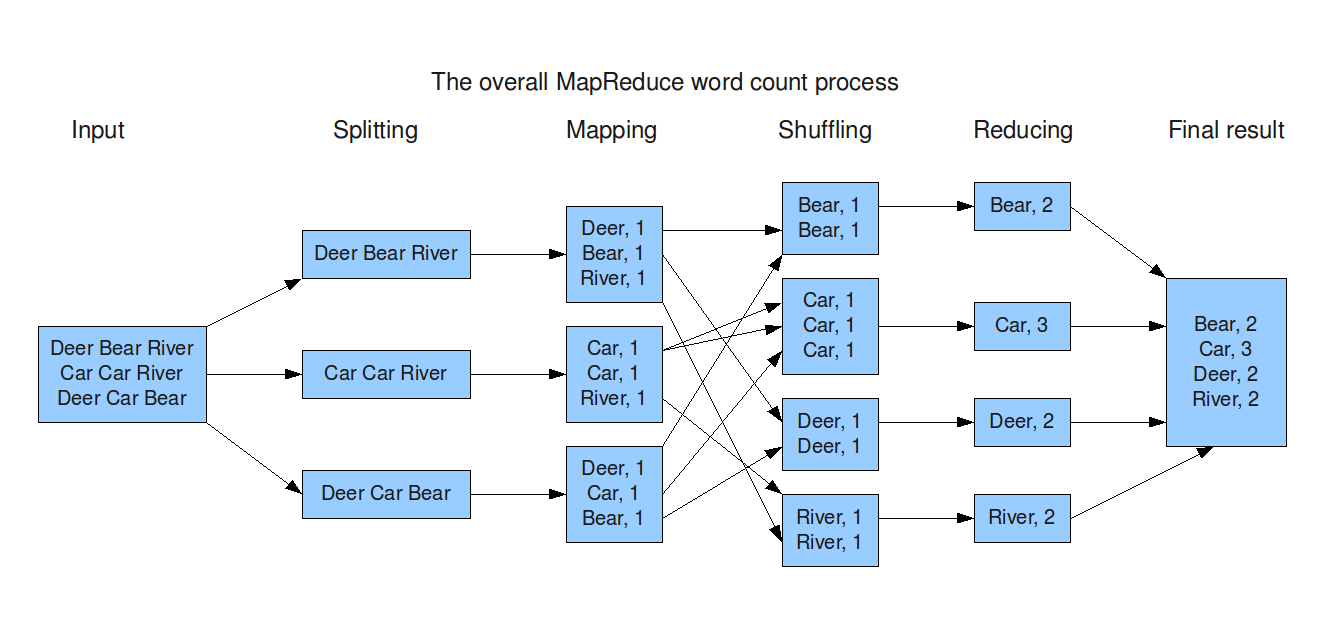
\includegraphics[width=3.8in]{mr.png}
\end{multicols}
\end{document}
